\documentclass[11pt]{article}
\usepackage{hyperref}
\urlstyle{same}
\usepackage{amsmath}
\usepackage{booktabs}
\usepackage{subcaption}
\usepackage{graphicx}
\usepackage{minted}
\usemintedstyle{tango}
\usepackage{inconsolata}
%\usepackage[T1]{fontenc}
\setcounter{secnumdepth}{-1}
\widowpenalty=100
\clubpenalty=100

\title{Programming languages and\\collaboration communities on GitHub}
\author{Corey Ford}

\begin{document}
\maketitle

\section{Introduction}

The website GitHub facilitates collaborative software development and hosts the
source code repositories, as well as other development activities, of numerous
open-source software projects, many of them widely-known.

To what extent does the diversity of programming language fragment the software
development community? We anticipate that the frequency of collaboration between
projects using the same programming language (or software framework, especially)
will result in communities identified by a programming language.

We construct the one-mode network of repositories, identify important
repositories in this network, and examine its community structure, comparing
communities defined by programming languages to those determined by common
community-detection algorithms.

\section{Related Work}
Some recent analyses have examined the programming languages associated with
each user via their repositories to determine conditional probabilities
\cite{doll12} or correlations \cite{shah13} relating to use of language pairs.

User communities based on primary programming languages and ``follower''
relationships were explored in \cite{cuny10,weber12}.  A visualization of the
bipartite graph of organizations (groups of users) and languages
\cite{rodrigues12} won third place in the 2012 GitHub Data Challenge.

Important nodes in the one-mode project-project and user-user networks, weighted
simply by number of common links, were identified in \cite{thung2013}.

\section{Methodology}
Data was obtained using SQL queries against the Google BigQuery web interface.
Further analysis was performed using Python 2.7 and version 0.6.5 of the igraph
library, and visualizations were created using Gephi 0.8.2 and sigma.js. All SQL
and Python code, along with data files, is available at
\url{https://github.com/coyotebush/github-network-analysis}.

\section{Data Collection}
We queried the GitHub Archive dataset\cite{githubarchive} to obtain data on
GitHub repositories that had received at least 1000 ``stars'' (a way for users
to bookmark interesting repositories) as of the end of 2012, including the URL,
primary programming language, and number of stars for each repository.

Using a second query, we computed a set of weighted edges between these
repositories based on two types of events: \emph{pushes}, where a user adds new
changes to a repository, and \emph{pull-request merges}, where a user without
push access proposes changes that are then reviewed and added to the repository
by another user who does.\footnote{Accounting only for pushes gave a relatively
disconnected graph, presumably because, as examined in \cite{khadke}, most users
have push access to only a few related repositories.  Including other types of
events, or measures such as lines of code, might produce different results, but
there is no definitive measure of developer productivity.} We first computed
contribution weights $C_{ui}$ for user-repository pairs as the number of times
the user has either pushed to or had a pull-request accepted to the repository
during 2012.\footnote{This counts pull-request merges for both the user who
submitted the request and the user who pushed the merge; this seems acceptable,
since it accounts for the work of reviewing a pull-request and better identifies
repository maintainers.}

Weights between repositories were then computed by examining users who have
contributed to each of a pair of repositories, and defining the weight of the
edge between repositories $i$ and $j$ as the sum over all users who have
contributed to both of the geometric mean of the number of times they have
contributed to each. The geometric mean was chosen because it is high when the
counts of a user's contributions to both repositories are high, but low when
either is low (and elegantly zero when they have not contributed at all to
either), and the impact of increasing either is diminishing. That is, the the
weights are defined by $W_{ij} \equiv \sum_u \sqrt{C_{ui} \cdot C_{uj}}$,
where $C$ is the contribution weight defined previously and $u$ ranges over all
GitHub users.\footnote{This is similar to the approach of \cite{marrama}, which
effectively used $\sqrt{min(C_{ui}, C_{uj})}$; \cite{opsahlproj,opsahl11}
provide additional insight into projections of such two-mode networks.}

The resulting graph contains 825 nodes and 3661 edges. However, for the
remainder of the analysis we consider only the giant component of this graph,
which contains 632 nodes and 3644 edges. This is justified by the lack of
meaningful structure in the remainder of the graph---the remaining connected
components comprise at most 3 nodes each---and reduces clutter both in the
visualization (which would have many nodes floating at the edge) and the
community detection (which would identify most of these nodes as their own
communities).

\section{Visualization}
A visualization of the network using the ForceAtlas 2 layout algorithm, with
nodes colored according to programming language and sized according to number of
stars, is shown in figure~\ref{fig:fullnetwork}. An interactive version is
available at \url{http://coyotebush.github.io/github-network-analysis/}.

\begin{figure}[htbp]
    \centering
    \caption{GitHub repository network.}
    \label{fig:fullnetwork}
    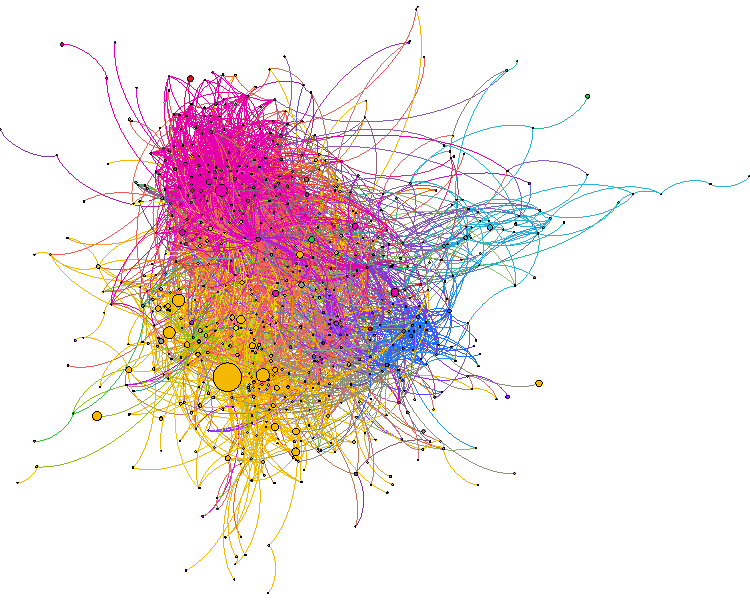
\includegraphics{repositories.pdf}
\end{figure}

Some language-based communities are already visually evident, including
\begin{itemize}
    \item Ruby (pink), which is noticeably centered around the prominent Ruby on
        Rails project (figure~\ref{fig:ruby}).
    \item JavaScript (yellow), the most popular language on GitHub and fairly
        central to this network.
    \item Python (blue).
    \item Objective-C (teal), which is relatively sparse.
\end{itemize}

\begin{figure}[htbp]
    \centering
    \caption{Ruby network.}
    \label{fig:ruby}
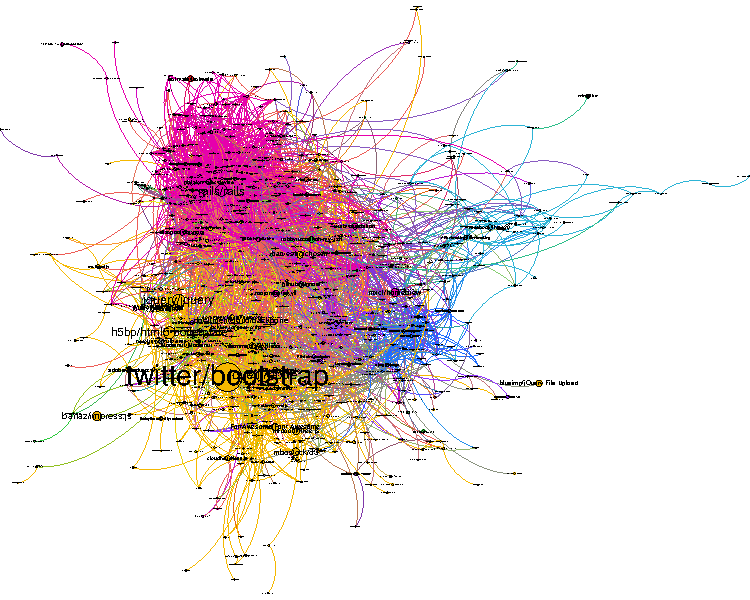
\includegraphics[clip=true,trim=1in 2.25in 2.5in 0.5in,scale=2]{repositories-labeled.pdf}
\end{figure}

\section[Analysis]{Analysis\footnote{This section was created using Pweave
(\url{http://mpastell.com/pweave/}) and
matrix2latex (\url{http://code.google.com/p/matrix2latex/})}}

\subsection{Notable repositories}

\input{analysis-repos.tex}

\subsubsection{Discussion}
Clearly, `rails/rails', the Ruby on Rails web application framework, is a very
important project on GitHub. This makes sense considering the strong community
of Rails plugins on GitHub, and that GitHub itself uses Rails.

Many of the other repositories in tables~\ref{tab:degree}, \ref{tab:between},
and \ref{tab:betweenw} (excluding `mperham/sidekiq' and `visionmedia/mocha')
serve as development tools moreso than as independent frameworks/applications,
so their importance is likely due to their use by developers who primarily code
in other languages.

Weighted degree (table \ref{tab:degreew}), which best represents the amount of
collaboration surrounding a project, includes none of these. From the
visualization, collaboration surrounding the two `ajaxorg' projects appears to
be primarily between the two, and the other three are web application
frameworks.

\subsection{Communities Defined by Language}

\input{analysis-languages.tex}

\subsubsection{Discussion}
The modularity resulting from clustering by language indicates significant
community structure, especially in the weighted version, which considers amount
of collaboration rather than merely its existence.

Among the top languages, the subgraph statistics for competing languages Ruby,
Python and PHP are notable. Although there are also many popular projects using
Objective-C and Java, their lower clustering coefficients reflect the perhaps
less open culture associated with these languages. JavaScript projects are
abundant but loosely connected. The Shell network is quite sparse; again, most
of these are probably development tools.

\subsection{Languages in Detected Communities}

\input{analysis-communities.tex}

\subsubsection{Discussion}
Both of these algorithms find a clustering with very high modularity.
\footnote{The Girvan-Newman edge-betweenness algorithm
(\texttt{community\_edge\_betweenness}), in addition to being very
computationally expensive, at best found a modularity of $0.290$, or $0.347$ for
the weighted version.} While Infomap more cautiously finds smaller communities,
in both cases most of the largest communities contain a majority of one of the
top programming languages in the dataset. This suggests that collaboration
communities do, in large part, form around languages. Some intra-language
collaboration is also evident, especially related to JavaScript; this might be
explained by JavaScript's use as a secondary, client-side language in web
applications written in another language.

\section{Conclusions}
On analyzing the network of collaboration between top GitHub repositories, we
find that programming language use is a reasonable indicator of community
structure, and vice versa. Still, there is plenty of collaborative activity
between projects using different languages.

A more complete picture might be obtained by lowering the threshold for
including repositories, thereby including less popular side projects, or by
changing the time range under consideration. Further work might also more
carefully analyze the relationships between languages themselves, ideally
incorporating data on non-primary languages used in a project.

\section{Acknowledgements}
This project is being developed both as the final project for a course in social
network analysis \cite{snacourse}, and as an entry in the GitHub Data Challenge
\cite{doll13}.

Thanks to Peter Faiman and Corey Farwell for help regarding SQL and
visualization, respectively.

{\small
\bibliographystyle{plain}
\bibliography{github}
}

\end{document}
% vim: ts=4 sts=4 sw=4 et tw=80
